%%%%%%%%%%%%%%%%%%%%%%%%%%%%%%%%%%%%%%%%%
% Focus Beamer Presentation
% LaTeX Template
% Version 1.0 (8/8/18)
%
% This template has been downloaded from:
% http://www.LaTeXTemplates.com
%
% Original author:
% Pasquale Africa (https://github.com/elauksap/focus-beamertheme) with modifications by 
% Vel (vel@LaTeXTemplates.com)
%
% Template license:
% GNU GPL v3.0 License
%
% Important note:
% The bibliography/references need to be compiled with bibtex.
%
%%%%%%%%%%%%%%%%%%%%%%%%%%%%%%%%%%%%%%%%%

%----------------------------------------------------------------------------------------
%	PACKAGES AND OTHER DOCUMENT CONFIGURATIONS
%----------------------------------------------------------------------------------------

\documentclass{beamer}

\usetheme{focus} % Use the Focus theme supplied with the template
% Add option [numbering=none] to disable the footer progress bar
% Add option [numbering=fullbar] to show the footer progress bar as always full with a slide count

% Uncomment to enable the ice-blue theme
%\definecolor{main}{RGB}{92, 138, 168}
%\definecolor{background}{RGB}{240, 247, 255}

%------------------------------------------------

\usepackage{booktabs}
\usepackage{longtable}
\usepackage{multirow}
\usepackage{colortbl}

%----------------------------------------------------------------------------------------
%	 TITLE SLIDE
%----------------------------------------------------------------------------------------

\title{Elixir Records}

\subtitle{Programming Scalabale Systems}

\author{Jorge Sol Gonzalez \\ Paula Pousa Martinez}

\institute{jorge.sol.gonzalez@alumnos.upm.es \\ paula.pousam@alumnos.upm.es}

\date{\today}

\titlegraphic{
\includegraphics[scale=0.20]{Images/elixir.png}}

%------------------------------------------------

\begin{document}

%------------------------------------------------

\begin{frame}
	\maketitle % Automatically created using the information in the commands above
\end{frame}

% Decisiones principales
%   Que hemos implementade, y "arquitectura" bdd y blockchain
% Dificultades encontradas
%   libreria ABI y Blockchain da error, la de herranz también
%   arrancar el GenServer
%   quorum no mola
% Herramientas utilizadas
%   exw3 para hacer llamadas
%   dificultad al recuperar eventos
%   o cualquier valor del smart contract, falta madurez de las librerias para esta tecnología


%------------------------------------------------

\begin{frame}{¿Qué es Elixir Records?}
	\begin{block}{Objetivo}
		Aplicacion web para registrar la asistencia de usuarios a eventos.
	\end{block}
  \begin{center}
  
\includegraphics[scale=0.5]{Images/logo.png}
  \end{center}
\end{frame}

\begin{frame}{Arquitectura del Proyecto}
  \begin{center}
  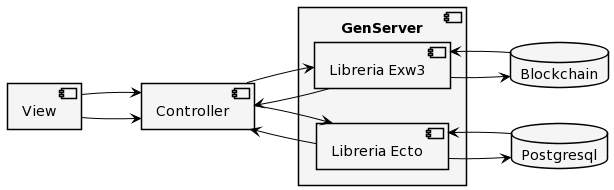
\includegraphics[scale=0.5]{Images/arquitectura.png}
  \end{center}
\end{frame}

%------------------------------------------------


\begin{frame}{Error keccakf1600}
  \begin{itemize}
    \item \textbf{ABI}: keccakf1600\_orig ~> 2.0.0 (app: keccakf1600)
    \item \textbf{Blockchain}: keccakf1600\_orig ~> 2.0.0 (app: keccakf1600)
  \end{itemize}
  \begin{center}
  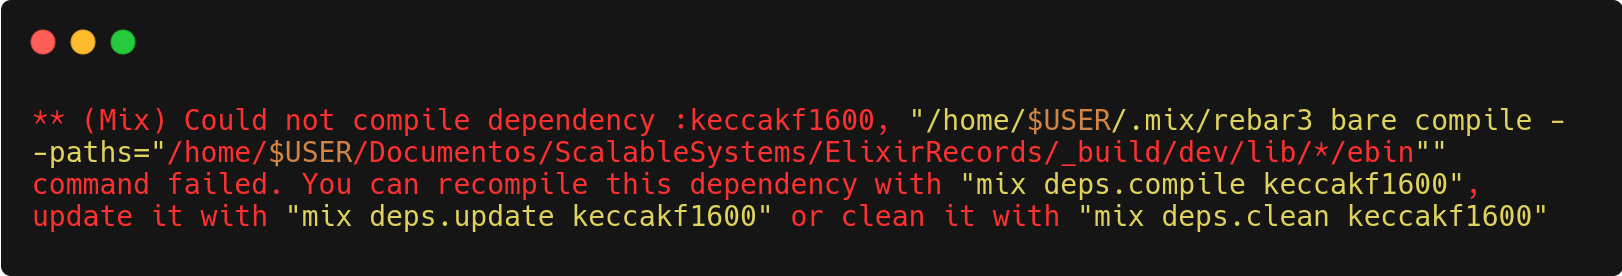
\includegraphics[scale=0.20]{Images/error.png}
  \end{center}
\end{frame}

\begin{frame}{Elixir Workers}
  \begin{center}
  
\includegraphics[scale=0.5]{Images/worker.png}
  \end{center}
\end{frame}

%------------------------------------------------

\begin{frame}{Herramientas Utilizadas}
  \begin{itemize}
    \item \textbf{Ecto}: Comunicación con la base de datos \textit{Postgresql}.
    \item \textbf{Exw3}: Comunicación con la red blockchain de \textit{Ganache}.
    \item \textbf{GenServer}: Comunicación entre el cliente y los distintos servicios.
    \item \textbf{Milligram}: Para el \textit{estilo} de la página web.
  \end{itemize}
\end{frame}

\begin{frame}{Librería Exw3}
	\begin{exampleblock}{\small Pros}
    \begin{itemize}
      \item {\small Permite las funcionalidades básicas}
        \begin{itemize}
          \item {\small Desplegar Smart Contracts}
          \item {\small Crear usuarios}
          \item {\small Interactuar con el Smart Contract}
          \item {\small Mandar Transacciones}
        \end{itemize}
      \item {\small Fácil de utilizar}
      \item {\small Trae las dependencias necesarias de facto}
    \end{itemize}
	\end{exampleblock}
	\begin{alertblock}{\small Contras}
    \begin{itemize}
      \item {\small Falta de documentación}
      \item {\small Funciones implementadas que aparentemente no funcionan}
      \item {\small Solo compatible con redes de Ethereum}
      \item {\small Parece imposible recuperar eventos}
    \end{itemize}
	\end{alertblock}
\end{frame}

\begin{frame}
  \begin{center}
  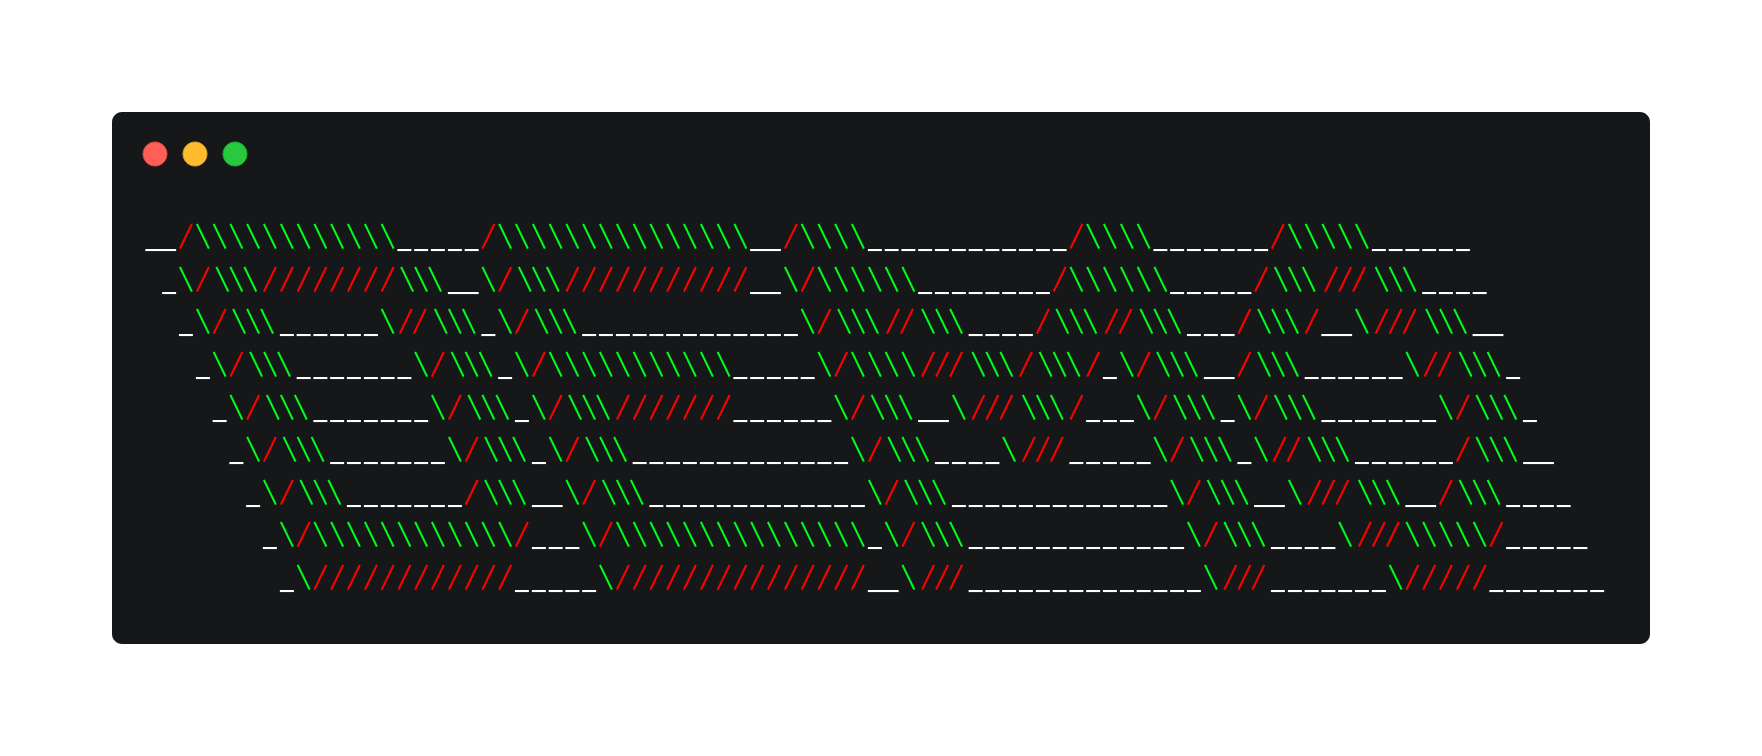
\includegraphics[scale=0.15]{Images/demo.png}
  \end{center}
\end{frame}

\end{document}
